% ============================================================
%  面向模拟可信执行环境的轻量级密钥管理系统设计与实现
%  本科毕业论文 / 技术报告 —— 初稿
%
%  编译方式（需 TeX Live / MiKTeX，含 ctex）：
%     xelatex main.tex
%     xelatex main.tex      % 第二次：生成目录、图表索引与交叉引用
%
%  说明：本模板为通用 ctexbook 排版，便于替换为所在院校的论文模板；
%        各章正文位于 chapters/ 下，可直接 \input 到院校模板中复用。
%  系统边界：Enclave 为软件模拟 TEE，非硬件 SGX，非生产级 KMS。
% ============================================================
% fontset=fandol：使用可自动下载的开源中文字体，跨引擎（tectonic / TeX Live）最稳。
% 若想用 macOS 系统字体（宋体等），把 fontset=fandol 改为 fontset=mac。
\documentclass[UTF8, fontset=fandol, a4paper, 12pt, openany, oneside]{ctexbook}

% ============================================================
%  preamble.tex —— 宏包、全局样式与自定义命令
%  编译：xelatex（需 ctex；建议 xelatex 连续编译两次以生成目录/交叉引用）
% ============================================================

% --- 页面 ---
\usepackage{geometry}
\geometry{a4paper, left=3cm, right=3cm, top=3cm, bottom=3cm}

% --- 数学与符号 ---
\usepackage{amsmath}
\usepackage{amssymb}

% --- 图形与表格 ---
\usepackage{graphicx}
\usepackage{booktabs}
\usepackage{longtable}
\usepackage{tabularx}
\usepackage{array}
\usepackage{multirow}
\usepackage{float}
\usepackage{caption}

% --- 列表 ---
\usepackage{enumitem}
\setlist{nosep, leftmargin=2.2em}

% --- 颜色与代码 ---
\usepackage{xcolor}
\usepackage{listings}

% --- 绘图 ---
\usepackage{tikz}
\usetikzlibrary{positioning, arrows.meta, shapes.geometric, fit, backgrounds, calc, automata}

% --- 超链接（放在较后）---
\usepackage[hidelinks]{hyperref}

% --- 下划线在正文中正常显示（避免大量 \_ 转义）；须在 hyperref 之后加载 ---
\usepackage{underscore}

% --- 行距 ---
\linespread{1.4}

% --- 图表编号按“章-序号”，标签与标题间用空格（中文习惯：图 4-1 标题）---
\renewcommand{\thefigure}{\thechapter-\arabic{figure}}
\renewcommand{\thetable}{\thechapter-\arabic{table}}
\renewcommand{\theequation}{\thechapter-\arabic{equation}}
\captionsetup{labelsep=space, font=small}

% --- 表格列类型 ---
\newcolumntype{Y}{>{\raggedright\arraybackslash}X}
\newcolumntype{C}[1]{>{\centering\arraybackslash}p{#1}}
\newcolumntype{L}[1]{>{\raggedright\arraybackslash}p{#1}}

% --- 代码样式 ---
\definecolor{codebg}{RGB}{248,248,248}
\definecolor{codekw}{RGB}{0,0,170}
\definecolor{codecmt}{RGB}{0,120,0}
\definecolor{codestr}{RGB}{160,0,0}
\definecolor{rulegray}{gray}{0.6}
\lstset{
  basicstyle=\ttfamily\footnotesize,
  backgroundcolor=\color{codebg},
  keywordstyle=\color{codekw}\bfseries,
  commentstyle=\color{codecmt},
  stringstyle=\color{codestr},
  numberstyle=\tiny\color{gray},
  breaklines=true,
  breakatwhitespace=false,
  showstringspaces=false,
  frame=single,
  rulecolor=\color{rulegray},
  columns=fullflexible,
  keepspaces=true,
  tabsize=2,
}

% --- 行内代码 ---
\newcommand{\code}[1]{\texttt{#1}}

% --- 带圈数字（①② 在拉丁/中文字体中可能缺字，统一用此宏绘制）---
\newcommand{\cnum}[1]{\textcircled{\raisebox{0.3pt}{\scriptsize #1}}}

% --- 减少 overfull：允许段落末行轻微伸展 ---
\emergencystretch=2em

% --- TikZ 通用样式 ---
\tikzset{
  box/.style   ={draw, rounded corners, align=center, inner sep=5pt,
                 minimum height=9mm, font=\small, fill=white},
  db/.style    ={draw, cylinder, shape border rotate=90, aspect=0.25,
                 align=center, inner sep=4pt, font=\footnotesize, fill=white},
  zone/.style  ={draw, dashed, rounded corners, inner sep=8mm},
  flow/.style  ={-{Stealth[length=2.5mm]}, thick},
  flowbi/.style={{Stealth[length=2.5mm]}-{Stealth[length=2.5mm]}, thick},
  lbl/.style   ={font=\footnotesize, align=center},
}


\ctexset{
  chapter/name   = {第,章},
  chapter/number = \arabic{chapter},
}

\title{\bfseries 面向模拟可信执行环境的\\轻量级密钥管理系统设计与实现}
\author{（作者姓名）\\[2mm] \large 指导教师：（教师姓名）}
\date{\today}

\begin{document}

% ---------------- 前置部分 ----------------
\frontmatter
\pagestyle{plain}

\maketitle

% ==================== 摘要 ====================
\chapter*{摘要}
\addcontentsline{toc}{chapter}{摘要}
\markboth{摘要}{摘要}

密钥管理是密码系统工程中最易出错的环节：密码算法本身相对成熟，但密钥的生成、存储、使用、轮换与销毁仍面临诸多工程挑战。在云环境与多租户等不可信主机（Host）场景下，若密钥管理系统（KMS）将主密钥与业务接口置于同一进程，一旦该进程被攻破，其保护的全部数据加密密钥将面临泄露风险。

针对上述问题，本文设计并实现了一套 Host 与 Enclave 分离的轻量级密钥管理系统。系统采用信封加密构建“主密钥—数据密钥—业务数据”的三层结构，将主密钥的持有、数据密钥的包装与解包以及数据加解密等敏感操作迁移至模拟可信执行环境（TEE）的 Enclave 进程；Host 仅负责鉴权、访问控制、密钥元数据管理与审计，数据库中仅保存包装后的数据密钥与业务密文。Host 与 Enclave 之间通过远程认证建立会话密钥，并在其上使用 AES-256-GCM 加密信道，配合序列号实现防重放。系统基于 Python 与 FastAPI 实现，提供 JWT 鉴权、基于角色的访问控制（RBAC）、版本化密钥轮换与审计日志，并以一个一键启动脚本完成 Host 与 Enclave 的联合部署。

本文建立了系统的威胁模型与安全需求，逐项给出已实现的缓解机制，并诚实界定了系统边界：本文 Enclave 为软件模拟而非硬件隔离，远程认证为结构性模拟，系统不防护物理攻击、侧信道以及 Enclave 自身被攻破等威胁。八项自动化集成测试验证了本地模式与可信模式下的鉴权、密钥生命周期、加解密往返与密钥轮换等功能的正确性。结果表明，在“Host 不可信、Enclave 相对可信”的受控威胁模型下，本方案能够将主密钥与数据密钥的敏感操作隔离至 Enclave，为后续对接真实硬件 TEE 与后量子密钥封装提供了可扩展的工程原型。

\vspace{1em}
\noindent\textbf{关键词：}密钥管理系统；信封加密；可信执行环境；远程认证；AES-GCM；应用密码学

% -------------------- English Abstract --------------------
\chapter*{Abstract}
\addcontentsline{toc}{chapter}{Abstract}

Key management is the most error-prone part of cryptographic engineering: while cryptographic algorithms are relatively mature, the generation, storage, use, rotation, and destruction of keys remain challenging. In cloud and multi-tenant settings where the host is not fully trusted, a Key Management System (KMS) that keeps the master key in the same process as its business API exposes all derived data encryption keys once that process is compromised.

To address this, this thesis designs and implements a lightweight KMS based on a Host/Enclave separation. The system uses envelope encryption to build a three-tier hierarchy of master key, data encryption key (DEK), and business data. Sensitive operations---holding the master key, wrapping and unwrapping DEKs, and performing data encryption/decryption---are moved into an Enclave process that simulates a Trusted Execution Environment (TEE). The Host is responsible only for authentication, access control, key metadata management, and auditing; the database stores only wrapped DEKs and ciphertext. The Host and the Enclave establish a session key through remote attestation and communicate over an AES-256-GCM channel with sequence numbers for replay protection. The prototype is implemented in Python with FastAPI, providing JWT authentication, role-based access control (RBAC), versioned key rotation, and audit logging, together with a one-command launch script that deploys the Host and the Enclave jointly.

This thesis establishes a threat model and a set of security requirements, maps each requirement to an implemented mitigation, and honestly delineates the system boundary: the Enclave is a software simulation rather than hardware isolation, the remote attestation is a structural simulation, and the system does not defend against physical attacks, side channels, or compromise of the Enclave itself. Eight automated integration tests verify the correctness of authentication, key lifecycle, encryption/decryption round-trips, and key rotation in both the local and the trusted modes. The results show that, under a controlled threat model where the host is untrusted and the Enclave is relatively trusted, the proposed design isolates sensitive master-key and DEK operations within the Enclave, providing an extensible engineering prototype for future integration with real hardware TEEs and post-quantum key encapsulation.

\vspace{1em}
\noindent\textbf{Keywords:} Key Management System; Envelope Encryption; Trusted Execution Environment; Remote Attestation; AES-GCM; Applied Cryptography


\tableofcontents
\listoffigures
\listoftables

% ---------------- 正文部分 ----------------
\mainmatter

% ==================== 第 1 章 绪论 ====================
\chapter{绪论}
\label{ch:intro}

\section{研究背景与动机}

随着信息系统对数据机密性要求的不断提高，密码学已成为现代软件系统的基础设施。然而，密码工程的实践经验反复表明：系统的安全性往往并不取决于所选密码算法的强度，而取决于密钥能否在其整个生命周期中得到妥善管理。换言之，密码算法相对成熟，真正的工程难点在于密钥的生成、存储、使用、轮换与销毁。美国国家标准与技术研究院（NIST）在其密钥管理建议中明确指出，密钥管理是密码系统中最复杂且最易出错的部分之一\cite{nist80057}。

密钥管理系统（Key Management System, KMS）正是为应对这一难题而生。它集中管理密钥的全生命周期，向上层应用提供加解密、密钥轮换等服务，并通过访问控制与审计保证密钥使用的合规性。在云计算与多租户场景中，KMS 已成为各大云服务商的核心安全组件。然而，KMS 自身的安全性高度依赖其运行环境：当承载 KMS 的主机（Host）不可信时——例如主机操作系统被攻破、运维人员越权访问，或进程内存遭到窥探——若主密钥（Master Key）与业务 API 处于同一进程，攻击者一旦控制该进程，便可读出主密钥，进而解密其保护的全部数据加密密钥（DEK），造成系统性的数据泄露。

为缩小这一暴露面，可信执行环境（Trusted Execution Environment, TEE）提供了一条可行路径。TEE 通过硬件机制在不可信的主机之上划出一块“小范围可信计算基（Trusted Computing Base, TCB）”，使其中的代码与数据即便面对拥有更高权限的攻击者也能保持机密性与完整性\cite{sabt2015tee}。Intel SGX、ARM TrustZone 等技术正是这一思想的代表\cite{costan2016sgx, pinto2019trustzone}。将密钥的敏感操作放入 TEE，可在 Host 失陷时仍保护主密钥不被窃取。本文正是沿此思路，探索在 Host 不可信前提下的轻量级 KMS 设计与实现。

\section{问题定义}

本文研究的核心问题可表述为：

\begin{quote}
\itshape 在 Host 不可信的前提下，如何设计并实现一套可运行的密钥管理系统，使主密钥与数据密钥的敏感操作不暴露在 Host 的内存与环境中？
\end{quote}

该问题包含三个相互关联的子问题：其一，如何组织密钥层次，使主密钥的暴露面最小化；其二，如何将敏感密码操作隔离至可信组件，并保证 Host 与可信组件之间通信的机密性、完整性与抗重放；其三，如何在保证上述安全目标的同时，提供完整的密钥生命周期管理、访问控制与审计能力。

需要特别说明的是，受限于本科毕业设计的资源与目标，本文不依赖真实硬件 TEE，而是以一个独立进程对 TEE 的关键能力（隔离执行、远程认证、安全信道）进行\textbf{软件模拟}。因此本文在追求设计完整性的同时，将始终明确区分“硬件 TEE 所能提供的保证”与“软件模拟所能提供的保证”，避免对原型能力的过度表述。

\section{研究目标}

围绕上述问题，本文设定如下研究目标：

\begin{enumerate}
  \item 设计“主密钥 $\rightarrow$ 数据密钥 $\rightarrow$ 业务数据”的两层密钥结构，并以信封加密实现。
  \item 实现密钥的全生命周期管理，包括创建、轮换、禁用、吊销与销毁。
  \item 将主密钥的持有与数据加解密等敏感操作迁移至模拟 Enclave，使其不出现在 Host 中。
  \item 建立 Host 与 Enclave 之间的远程认证与安全通信协议。
  \item 提供 JWT 鉴权、基于角色的访问控制与审计日志，并给出可复现的原型与自动化测试。
\end{enumerate}

\section{主要贡献}

本文的主要贡献概括如表~\ref{tab:contrib} 所示。

\begin{table}[H]
\centering
\caption{本文主要贡献}
\label{tab:contrib}
\small
\begin{tabularx}{\textwidth}{cY}
\toprule
编号 & 贡献 \\
\midrule
1 & 设计并实现了一套轻量级 KMS 架构，集成 RBAC、审计与版本化密钥轮换。 \\
2 & 提出并实现了 Host/Enclave 分离的信封加密方案，使明文数据密钥不出 Enclave。 \\
3 & 实现了简化的远程认证与基于 AES-GCM 的会话信道，并支持序列号防重放。 \\
4 & 建立了系统的威胁模型与安全需求，并诚实界定了软件模拟 TEE 的能力边界。 \\
5 & 提供了可一键启动的原型系统与八项自动化集成测试，保证结果可复现。 \\
\bottomrule
\end{tabularx}
\end{table}

\section{论文组织结构}

本文共分八章，组织如下：第~\ref{ch:intro}~章为绪论，介绍研究背景、问题与目标；第~\ref{ch:background}~章综述相关技术与理论基础，包括认证加密、信封加密、KMS、TEE 与访问控制；第~\ref{ch:threat}~章建立系统的威胁模型与安全需求；第~\ref{ch:design}~章给出系统总体设计，包括架构、密钥层次、模块划分与数据模型；第~\ref{ch:protocol}~章详述关键协议与算法实现，包括远程认证握手与加解密全链路时序；第~\ref{ch:impl}~章介绍系统实现与部署；第~\ref{ch:eval}~章给出测试与实验评估；第~\ref{ch:conclusion}~章总结全文并展望未来工作。

% ==================== 第 2 章 相关技术与理论基础 ====================
\chapter{相关技术与理论基础}
\label{ch:background}

本章综述本文所依赖的核心技术与理论，为后续章节的设计与实现奠定基础。内容涵盖对称密码与认证加密、密钥派生与信封加密、密钥管理系统、可信执行环境以及身份认证与访问控制五个方面，并在每一方面指出本文的具体取舍。

\section{对称密码与认证加密}
\label{sec:aead}

对称密码使用同一密钥进行加密与解密，具有运算高效的特点，适合加密大量数据。然而，仅保证机密性的加密模式（如 CBC）无法抵御密文篡改，历史上由此产生了诸如填充预言（padding oracle）等攻击。认证加密（Authenticated Encryption with Associated Data, AEAD）在加密的同时提供完整性与真实性保证，并允许将一段“关联数据”绑定到密文上参与完整性校验，但该关联数据本身不被加密\cite{rogaway2002aead, rfc5116}。

本文统一采用 AES-256-GCM 作为认证加密算法\cite{fips197, dworkin2007gcm, mcgrew2004gcm}。GCM（Galois/Counter Mode）在计数器模式加密的基础上引入 GHASH 认证，输出密文与一个认证标签（tag）；解密时若标签校验失败则拒绝输出明文，从而同时保证机密性与完整性。使用 GCM 时需特别注意两点：其一，随机数（nonce）在同一密钥下必须唯一，nonce 重用会严重削弱安全性，因此本文在每次加密时均生成新的 96 位随机 nonce；其二，关联数据可用于将密文与其使用上下文绑定，本文借此把数据密文与具体密钥身份绑定（详见第~\ref{ch:design}~章）。选择 GCM 而非 CBC 的根本原因即在于其 AEAD 特性，可一并解决机密性与完整性问题，并规避填充预言一类风险。

\section{密钥派生与信封加密}
\label{sec:envelope}

在实际系统中，直接用单一密钥加密所有数据会带来密钥暴露面过大、轮换困难等问题。信封加密（envelope encryption）通过分层结构缓解这一矛盾：系统持有一把高价值的主密钥（Master Key），用它“包装”（加密）若干数据密钥（Data Encryption Key, DEK），再以 DEK 加密业务数据。被包装后的 DEK 可安全地与密文一同存储，而主密钥仅用于包装/解包，使用频率与暴露面大大降低。这一模式被各大云 KMS 广泛采用\cite{nist80057}。

与系统密钥相关但目标不同的，是用户口令的处理。口令不应被加密存储，而应使用专门的口令哈希函数进行单向保护。本文对用户口令采用 bcrypt\cite{provos1999bcrypt}，它通过加盐与可调代价因子抵抗暴力破解；这与用于派生系统密钥的 PBKDF2\cite{rfc8018} 等密钥派生函数在用途上有本质区别——前者用于验证口令，后者用于生成密钥材料。明确区分“口令哈希”与“密钥派生/包装”是密钥管理工程中的基本原则。

\section{密钥管理系统}
\label{sec:kms}

密钥管理系统在公钥基础设施（PKI）与云安全中承担密钥全生命周期的集中管理职责。一个完整的密钥生命周期通常包括创建（Create）、使用（Use）、轮换（Rotate）、吊销（Revoke）与销毁（Destroy）等阶段\cite{nist80057}。轮换用于限制单把密钥的使用时长与数据量，吊销与销毁用于在密钥可能泄露或不再需要时及时止损；其中轮换需兼顾“新数据用新密钥”与“历史密文仍可解密”这一对看似矛盾的需求，通常通过保留密钥的历史版本来实现。

在产品形态上，KMS 可由硬件安全模块（HSM）提供最强的密钥隔离，也可由云 KMS（如各类公有云密钥服务）以托管方式提供弹性与易用性。本文实现的系统在定位上不同于上述生产级方案：它是一个面向教学与研究的\textbf{轻量级工程原型}，强调架构清晰、可复现与威胁模型的诚实表述，而非高可用、合规认证或硬件级隔离。第~\ref{ch:eval}~章将对本文系统与云 KMS 在功能、威胁模型与适用场景上作定性对比。

\section{可信执行环境}
\label{sec:tee}

可信执行环境（TEE）的基本思想是在不可信的主机环境中，借助硬件机制构造一块受保护的执行区域（通常称为 Enclave），使其中的代码与数据的机密性和完整性不依赖于操作系统或更高权限的软件\cite{sabt2015tee}。Intel SGX 通过受保护的内存区域（Enclave Page Cache）与一系列处理器指令实现隔离执行\cite{costan2016sgx, mckeen2013sgx}；ARM TrustZone 则通过将系统划分为“安全世界”与“普通世界”来隔离敏感计算\cite{pinto2019trustzone}。

TEE 的两项关键能力与本文密切相关。其一是\textbf{远程认证}（Remote Attestation）：Enclave 能够生成一份可被远端验证的、关于其自身代码与配置的度量证明，使验证方确信自己正在与一个预期的、未被篡改的 Enclave 通信；在 SGX 中这一过程涉及 \texttt{EREPORT}/\texttt{QUOTE} 等机制，并由硬件厂商的认证服务背书\cite{anati2013attestation}。其二是\textbf{密封存储}（Sealed Storage）：Enclave 可用与其身份绑定的密钥加密数据后存盘，使得只有相同度量值的 Enclave 才能解封。

\textbf{本文采用软件模拟 TEE。}具体而言，本文以一个独立的操作系统进程承载 Enclave，对隔离执行、远程认证与安全信道等能力进行结构性模拟：以代码度量值的比对模拟身份验证，以挑战-响应与会话密钥协商模拟认证握手，以 AES-GCM 信道模拟安全通信。必须强调，软件模拟与真实硬件 TEE 存在本质差异：模拟 Enclave 仍是普通进程，不具备硬件内存加密与隔离，其远程认证也不具备硬件根信任。这些差异构成本文系统的能力边界，将在第~\ref{ch:threat}~章作出明确声明。

\section{身份认证与访问控制}
\label{sec:authz}

KMS 必须严格控制“谁能对哪些密钥执行何种操作”。本文在身份认证层面采用基于 JWT（JSON Web Token）的 Bearer 令牌机制\cite{rfc7519}：用户登录后获得一个带签名与过期时间的令牌，后续请求通过携带该令牌完成无状态鉴权。令牌签名采用 HMAC-SHA256\cite{rfc2104, fips180}，其密钥由服务端持有。

在授权层面，本文采用基于角色的访问控制（Role-Based Access Control, RBAC），定义管理员（Admin）、密钥管理员（Key Manager）与应用用户（App User）三类角色，按角色限制接口访问权限（详见第~\ref{ch:design}~章的权限矩阵）。此外，审计日志记录关键操作的执行者、动作、目标与结果，为事后追溯与异常检测提供依据，是安全系统不可或缺的组成部分。

\section{本章小结}

本章梳理了本文所依赖的关键技术：以 AES-256-GCM 实现认证加密，以信封加密构建分层密钥结构，以密钥生命周期管理组织 KMS 功能，以 TEE 思想隔离敏感操作，并以 JWT、RBAC 与审计构建访问控制与可追溯能力。其中，本文对 TEE 采用软件模拟这一关键取舍贯穿全文，其能力边界将在下一章的威胁模型中被严格界定。

% ==================== 第 3 章 系统威胁模型与安全需求 ====================
\chapter{系统威胁模型与安全需求}
\label{ch:threat}

\begin{quote}\small
本章基于现有原型代码撰写，所述机制均对应已实现功能。系统边界：本文 Enclave 为软件模拟可信执行环境（TEE），非 Intel SGX 等硬件隔离，亦非生产级 KMS。本章在描述防护能力的同时，明确区分“已实现的缓解”与“假设/不在防护范围内的威胁”。
\end{quote}

\section{威胁建模方法与本章组织}

密钥管理系统的安全性不取决于单个密码算法的强度，而取决于密钥在其整个生命周期中是否始终处于受控状态。因此在进入具体设计之前，有必要先建立清晰的威胁模型，明确“在何种假设下、防护何种攻击者、达到何种安全目标”。本章采用面向资产的轻量级威胁建模流程，依次完成资产识别、角色与信任边界刻画、攻击者建模、威胁分析与缓解、系统边界声明，并最终导出可验证的安全需求清单。

需要说明的是，本章给出的是\textbf{设计级（design-level）威胁模型}，用于指导系统设计与测试，并非形式化的协议安全证明；形式化验证列入第~\ref{ch:conclusion}~章的未来工作。在威胁分类视角上，本章借鉴 STRIDE 中的信息泄露、篡改、假冒与权限提升等维度，但以“资产—威胁—缓解”的工程化表格形式呈现，以便与具体实现一一对应。

\section{资产识别}

系统的安全设计围绕密钥层次展开。表~\ref{tab:assets} 列出需要保护的核心资产、存放位置及敏感级别。其中主密钥（Master Key）是整个信封加密体系的信任根，一旦泄露将导致其保护的全部数据密钥（DEK）及业务数据失陷，故列为最高敏感级别。

\begin{table}[H]
\centering
\caption{关键资产清单}
\label{tab:assets}
\footnotesize
\begin{tabularx}{\textwidth}{c L{3.0cm} L{3.6cm} c Y}
\toprule
编号 & 资产 & 存放位置 & 敏感级别 & 泄露后果 \\
\midrule
A1 & 主密钥（L0，32 字节） & 仅 Enclave 进程内存（可信模式） & 极高 & 全部 DEK 与业务数据失陷 \\
A2 & 明文 DEK（L1，32 字节） & 仅在 Enclave 内临时存在 & 高 & 对应密钥下业务数据失陷 \\
A3 & 包装后的 DEK & 数据库 & 中 & 仅在同时获得主密钥时才有价值 \\
A4 & 业务明文 / 密文 & 客户端 / 数据库 & 中 & 单条业务数据泄露 \\
A5 & 口令哈希、JWT 签名密钥 & Host（bcrypt 哈希 / 环境变量） & 高 & 身份冒充、令牌伪造 \\
A6 & 审计日志 & 数据库 & 中 & 抵赖、痕迹清除 \\
A7 & 会话密钥、Enclave 身份密钥 & Host/Enclave 进程内存 & 高 & 信道被解密 / 冒充 \\
\bottomrule
\end{tabularx}
\end{table}

按敏感级别排序，系统设计的首要目标是保护 A1 与 A2，即\textbf{让主密钥与明文 DEK 不出现在 Host 环境中}；这正是引入模拟 Enclave 的根本动机。

\section{系统角色与信任边界}

\subsection{系统角色}

系统涉及以下参与方：\textbf{调用方（Client）}通过 HTTP 接口访问系统，凭 JWT 鉴权，分为 Admin、Key Manager、App User 三类；\textbf{Host（MiniKMS）}负责鉴权、RBAC、密钥元数据管理与审计，并在可信模式下\textbf{不持有}主密钥、\textbf{不解包} DEK；\textbf{数据库（DB）}保存元数据、包装后的 DEK、业务密文与日志，\textbf{不保存}主密钥与明文 DEK；\textbf{Enclave（KmsEnclave）}持有主密钥，负责生成/包装 DEK、解包 DEK 并在内部完成数据加解密，明文 DEK 不离开 Enclave；此外，\textbf{被动网络观察者/恶意运维}作为潜在攻击者纳入考虑。

\subsection{信任边界}

系统存在两条关键信任边界，如图~\ref{fig:trust} 所示。边界\cnum{1}（调用方 $\leftrightarrow$ Host）要求调用方通过 JWT 鉴权并受 RBAC 约束；边界\cnum{2}（Host $\leftrightarrow$ Enclave）是本文威胁模型的核心：在可信模式下，Host 被视为\textbf{对密钥机密性而言不可信}，主密钥被隔离在边界另一侧的 Enclave 中，二者通过本地 IPC 连接，并在其上叠加远程认证与 AES-GCM 加密信道。

\begin{figure}[H]
\centering
\resizebox{\textwidth}{!}{%
\begin{tikzpicture}[node distance=24mm]
  \node[box] (C) {客户端 / Swagger\\[1pt]\footnotesize Admin · Key Manager · App User};
  \node[box, right=of C] (H) {MiniKMS Host\\[1pt]\footnotesize FastAPI · JWT/RBAC · 审计};
  \node[box, right=of H] (E) {KmsEnclave\\[1pt]\footnotesize 包装/解包 DEK · AES-GCM};
  \node[db, below=16mm of H] (DB) {SQLite\\包装后 DEK\\密文 · 日志};
  \draw[flow]   (C) -- node[lbl, above]{\cnum{1} HTTP + JWT} (H);
  \draw[flowbi] (H) -- node[lbl, above]{\cnum{2} 远程认证\\+ AES-GCM 信道} (E);
  \draw[thick]  (H) -- (DB);
  \begin{scope}[on background layer]
    \node[zone, fit=(C),       label=below:{\footnotesize 调用方区域（不可信网络）}] {};
    \node[zone, fit=(H)(DB),   label=below:{\footnotesize Host 区域（可信模式下视为不可信）}] {};
    \node[zone, fit=(E),       label=below:{\footnotesize Enclave 区域（模拟可信 · 持有 Master Key）}] {};
  \end{scope}
\end{tikzpicture}}
\caption{系统信任边界与数据流}
\label{fig:trust}
\end{figure}

\subsection{信任假设}

本章威胁模型建立在以下假设之上：

\begin{itemize}
  \item \textbf{A-1（Enclave 相对可信）}：Enclave 进程未被攻破，其内存与执行流程不被外部读取或篡改。\textbf{此假设由模拟环境约定保证，而非硬件强制}——真实部署中需由 SGX 等硬件 TEE 提供，本文以独立进程加主密钥仅注入 Enclave 的方式进行结构性模拟。
  \item \textbf{A-2（Host 可能被攻破）}：可信模式下允许 Host 进程被控制或其内存/环境变量被窥探；设计目标是即便如此，主密钥与明文 DEK 也不落入攻击者之手。
  \item \textbf{A-3（数据库不可信）}：允许攻击者获得数据库文件的完整副本。
  \item \textbf{A-4（本地可信 IPC）}：Host 与 Enclave 部署于同一主机，经环回 TCP 或 Unix Domain Socket 通信；假设攻击者无法在该本地信道的\textbf{握手阶段}进行主动中间人攻击（必要性见第~\ref{sec:threat-analysis}~节 T4）。
  \item \textbf{A-5（合法用户经鉴权）}：所有业务接口调用者均须持有有效 JWT，且其角色受 RBAC 约束。
\end{itemize}

需强调，\textbf{本地模式}（\code{USE_ENCLAVE=false}）下主密钥位于 Host 的 \code{.env}，此时 Host 属可信区，A-2 不成立。本地模式仅用于开发与对照实验，本章以\textbf{可信模式为主要分析对象}，本地模式作为对照基线。

\section{攻击者模型}

综合上述资产与边界，本文考虑具备以下能力的攻击者：\textbf{C-1} 数据库泄露（读取或导出全部表内容）；\textbf{C-2} Host 进程窥探（读取 Host 内存、环境变量与配置）；\textbf{C-3} 被动窃听（监听调用方$\leftrightarrow$Host 流量，以及握手之后的 Host$\leftrightarrow$Enclave 信道）；\textbf{C-4} 主动篡改/重放（篡改或重放 Host$\leftrightarrow$Enclave 信道消息）；\textbf{C-5} 冒充 Enclave（以伪造或错误版本的 Enclave 应答）；\textbf{C-6} 越权调用（以合法低权限身份尝试越权操作）。不在攻击者能力范围内的情形统一在第~\ref{sec:boundary}~节声明。

\section{威胁分析与缓解措施}
\label{sec:threat-analysis}

针对上述攻击者能力，表~\ref{tab:threats} 给出系统已实现的缓解机制及对应代码位置。

\begin{table}[H]
\centering
\caption{威胁分析与缓解措施}
\label{tab:threats}
\footnotesize
\begin{tabularx}{\textwidth}{c L{3.3cm} Y L{3.4cm}}
\toprule
编号 & 威胁（攻击者能力） & 缓解机制 & 实现位置 \\
\midrule
T1 & C-1 数据库泄露 & DB 仅存包装后的 DEK 与业务密文，不含主密钥与明文 DEK；销毁时擦除包装材料 & \code{models/key.py}、\code{key_service.destroy_key} \\
T2 & C-2 Host 窥探（可信模式） & 主密钥仅在 Enclave；Host 配置强制将 \code{master_key} 置空；解包与加解密在 Enclave 内完成 & \code{config.py}、\code{crypto_service}、\code{enclave_client} \\
T3 & C-3 被动窃听 & Host$\leftrightarrow$Enclave 会话 AES-256-GCM 加密；调用方$\leftrightarrow$Host 假设由部署层 TLS 保护 & \code{enclave.py} 的安全收发 \\
T4 & C-4 篡改/重放 & 信道消息带 GCM 认证标签（篡改即失败）+ 单调递增序列号 \code{seq}（重放即拒） & \code{enclave_client.py}、\code{enclave.py} \\
T5 & C-5 冒充 Enclave & 远程认证：校验度量值 + 挑战-响应（HMAC）验证身份密钥 & \code{handle_attestation} 等 \\
T6 & C-6 越权调用 & JWT + RBAC；App User 仅能使用 active 密钥、不能管理密钥；越权写审计 & \code{utils/permissions.py}、各 \code{api/*.py} \\
T7 & 凭证泄露 & 口令仅存 bcrypt 哈希；响应从不返回密钥材料、口令哈希或主密钥 & \code{utils/security.py}、响应 schema \\
T8 & 解密错误旁路 & 解密/解包失败统一返回通用错误，不暴露内部细节 & \code{crypto_service}、\code{kms_enclave} \\
\bottomrule
\end{tabularx}
\end{table}

下面对若干关键威胁补充说明，并\textbf{诚实标注其残余风险}。

\textbf{T2（Host 被攻破时的密钥保护）。} 可信模式下，即使攻击者完全控制 Host 进程，也无法直接读出主密钥或离线导出明文 DEK——这是本方案相对纯本地模式的核心安全增益。但须指出其\textbf{残余风险}：在一个已建立的认证会话存续期间，被攻陷的 Host 仍可向 Enclave 提交加解密请求，即 Enclave 对持有该会话的一方而言是一个“加解密预言机（oracle）”。因此本方案的保护边界应准确表述为——\textbf{主密钥不被窃取、无法离线/规模化解密历史数据}，而非“Host 被攻破后数据绝对安全”。会话或 Enclave 终止后，攻击者即丧失该能力。

\textbf{T4 / T5（远程认证的真实强度）。} 当前远程认证可有效拒绝\textbf{版本错误或度量值不匹配的 Enclave}：Host 通过比对度量值（\code{SHA256("trusted-kms-enclave-v1.0")}）识别对端。但其密码学强度受模拟实现限制：身份密钥为\textbf{对称密钥且在握手阶段以明文传输}，会话密钥随后用该身份密钥加密下发。这意味着该认证\textbf{不能抵御能够观测并主动操纵握手过程的攻击者}——与真实 SGX 中由硬件根证书背书的非对称远程认证存在本质差异。故本文将其归类为\textbf{结构性模拟的远程认证}，并以假设 A-4 作为其成立前提。

\section{明确不在防护范围内的威胁（系统边界）}
\label{sec:boundary}

为避免对原型能力的过度表述，本节明确声明表~\ref{tab:boundary} 所列威胁\textbf{不在}本文防护范围内。这些边界主要源于“软件模拟 TEE”这一根本定位。

\begin{table}[H]
\centering
\caption{明确不在防护范围内的威胁}
\label{tab:boundary}
\footnotesize
\begin{tabularx}{\textwidth}{c L{4.8cm} Y}
\toprule
编号 & 不防护的威胁 & 原因说明 \\
\midrule
N1 & 物理攻击、冷启动、总线探测 & 软件模拟，无硬件隔离与内存加密 \\
N2 & 硬件/微架构侧信道（时序、缓存等） & 未做侧信道防护；不属本文主线 \\
N3 & Enclave 进程本身被攻破 & 模拟下 Enclave 为普通进程，主密钥驻留普通内存，具 root/调试/内存转储能力者可读取 \\
N4 & 同时控制 Host 与 Enclave 的攻击者 & 双端皆失陷时可在 Enclave 内解密，超出本模型 \\
N5 & 对远程认证握手的主动中间人 & 受对称明文身份密钥限制，依赖假设 A-4 \\
N6 & 调用方$\leftrightarrow$Host 的传输层加密（TLS） & 原型以 HTTP 运行，TLS 由部署层提供，未在原型实现 \\
N7 & 令牌被盗后的即时吊销 & JWT 在有效期内有效，未实现刷新令牌与吊销列表 \\
N8 & 细粒度/多租户密钥隔离 & 访问控制为角色级，任意已鉴权用户可用任意 active 密钥，无逐密钥 ACL \\
N9 & 拒绝服务（DoS）与可用性攻击 & 本文聚焦机密性与完整性，不以可用性为目标 \\
N10 & 供应链与依赖完整性 & 不在本文范围 \\
\bottomrule
\end{tabularx}
\end{table}

此外需补充：基类 \code{Enclave} 虽提供“加密内存”与“密封存储”等抽象，但 KMS 的主密钥路径并未经由加密内存存放，而是以普通进程内存中的密钥对象形式持有；Enclave 用完明文 DEK 后会将局部变量重置为零值，这属于\textbf{尽力而为的清零}，受 Python 运行时（不可变 \code{bytes} 与垃圾回收）限制，并非保证性的内存擦除。上述说明与“模拟 TEE、非生产级 KMS”的定位一致。

\section{安全需求}

综合前述分析，本文导出如下可验证的安全需求。SR1--SR6 为核心需求，SR7--SR8 为支撑性需求；每条均标注其针对的威胁与落实位置，便于在第~\ref{ch:eval}~章验证。

\begin{table}[H]
\centering
\caption{安全需求与落实位置}
\label{tab:sr}
\footnotesize
\begin{tabularx}{\textwidth}{c Y L{2.4cm} L{4.0cm}}
\toprule
编号 & 安全需求 & 对应威胁/资产 & 落实位置 \\
\midrule
SR1 & 可信模式下主密钥不得出现在 Host 环境变量或进程内存中 & T2 / A1 & \code{config.py} 强制 \code{master_key=None}；加解密转发 Enclave \\
SR2 & 每次数据加密使用新的随机 nonce（12 字节） & 机密性 / A4 & 加密路径调用 \code{os.urandom(12)} \\
SR3 & 解密失败返回统一错误，不泄露内部细节 & T8 & \code{crypto_service}、\code{kms_enclave} \\
SR4 & 密钥轮换后旧版本仍可解密历史密文 & 正确性 & \code{KeyVersion} 版本表 \\
SR5 & 销毁密钥后擦除数据库中的包装后密钥材料 & T1 / A3 & \code{key_service.destroy_key} \\
SR6 & 关键操作写入审计日志 & T6 / A6 & \code{audit_service.record_event} \\
SR7 & 接口访问遵循最小权限 & T6 & \code{require_roles} 与各路由依赖 \\
SR8 & Host$\leftrightarrow$Enclave 信道保证机密性、完整性并防重放 & T3/T4 & AES-GCM 会话加密 + \code{seq} 校验 \\
\bottomrule
\end{tabularx}
\end{table}

这些需求构成第~\ref{ch:design}~章系统设计的约束，也是第~\ref{ch:eval}~章测试用例的设计依据。需注意 SR1、SR8 的有效性以信任假设（尤其 A-1、A-4）为前提；脱离这些假设，相应保证不再成立。

\section{本章小结}

本章建立了系统的威胁模型与安全需求。首先识别了以主密钥为信任根的核心资产，随后刻画了系统角色与两条信任边界（图~\ref{fig:trust}），其中 Host$\leftrightarrow$Enclave 边界是本文将主密钥隔离至模拟 Enclave 的关键。在此基础上，本章界定了攻击者能力，逐项分析了数据库泄露、Host 窥探、信道篡改、冒充 Enclave、越权调用等威胁并对应到代码实现（表~\ref{tab:threats}）。更重要的是，本章以独立小节（第~\ref{sec:boundary}~节）诚实声明了系统边界，避免对原型能力的夸大，并导出了 SR1--SR8 的安全需求清单（表~\ref{tab:sr}），作为后续设计与测试的统一约束。

% ==================== 第 4 章 系统总体设计 ====================
\chapter{系统总体设计}
\label{ch:design}

\begin{quote}\small
本章描述系统的总体架构、密钥层次、模块划分、数据模型、API 与权限设计及密钥生命周期，均对应现有原型代码已实现的结构。涉及关键协议（远程认证、加解密时序）的细节在第~\ref{ch:protocol}~章展开，本章聚焦结构性设计。
\end{quote}

\section{设计目标与原则}

依据第~\ref{ch:threat}~章的威胁模型与安全需求（SR1--SR8），系统设计遵循以下原则：（1）\textbf{最小可信计算基}，将最敏感的密码操作集中到尽可能小的可信组件（Enclave），使 Host 即便失陷也无法获得主密钥（对应 SR1）；（2）\textbf{信封加密分层}，采用“主密钥 $\rightarrow$ 数据密钥 $\rightarrow$ 业务数据”三层结构，降低主密钥的使用频率与暴露面；（3）\textbf{关注点分离}，Host 负责编排、鉴权、策略与审计，Enclave 负责密码学执行；（4）\textbf{纵深防御}，在传输、鉴权、授权、加密、审计多层叠加控制；（5）\textbf{可对照、可降级}，提供本地与可信两种后端，共享同一套 API 与数据模型；（6）\textbf{诚实边界}，不以软件模拟冒充硬件隔离。

\section{总体架构}

系统采用 \textbf{Host + Enclave 分离}的三层架构，如图~\ref{fig:arch} 所示。自上而下分别为调用方、Host（MiniKMS）与 Enclave（KmsEnclave），数据库由 Host 管理。

\begin{figure}[H]
\centering
\resizebox{0.96\textwidth}{!}{%
\begin{tikzpicture}[node distance=8mm]
  \node[box] (C) {客户端 / Swagger};
  \node[box, below=14mm of C] (API) {API 路由层\\[1pt]\footnotesize auth · users · keys · crypto · audit};
  \node[box, below=8mm of API] (SVC) {服务层\\[1pt]\footnotesize auth · key · crypto · audit · enclave\_client};
  \node[db, right=16mm of SVC] (DB) {SQLite\\元数据 · 包装DEK\\密文 · 日志};
  \node[box, below=22mm of SVC] (OPS) {生成/包装/解包 DEK · AES-GCM 加解密};
  \node[box, below=7mm of OPS] (MK) {Master Key（仅驻留于此）};
  \draw[flow]   (C)   -- node[lbl, right]{\cnum{1} HTTP + JWT} (API);
  \draw[flow]   (API) -- (SVC);
  \draw[flow]   (SVC) -- node[lbl, above]{ORM} (DB);
  \draw[flowbi] (SVC) -- node[lbl, left, align=left]{\cnum{2} 远程认证 + AES-GCM 信道\\ kms\_generate\_wrapped\_dek\\ kms\_encrypt / kms\_decrypt} (OPS);
  \draw[flow]   (MK)  -- (OPS);
  \begin{scope}[on background layer]
    \node[zone, fit=(API)(SVC)(DB), label={[font=\footnotesize]right:Host：MiniKMS（不持有主密钥）}] {};
    \node[zone, fit=(OPS)(MK),      label={[font=\footnotesize]right:Enclave：KmsEnclave（模拟 TEE，可信区）}] {};
  \end{scope}
\end{tikzpicture}}
\caption{系统总体架构}
\label{fig:arch}
\end{figure}

各层职责如下：\textbf{调用方层}通过 HTTP 访问 RESTful 接口，所有业务请求携带 JWT 令牌；\textbf{Host 层（MiniKMS）}基于 FastAPI 实现，含 API 路由层与服务层，并以 JWT 鉴权、RBAC 与审计作为横切关注点，管理 SQLite 数据库，但在可信模式下\textbf{既不持有主密钥，也不在本进程内解包 DEK}；\textbf{Enclave 层（KmsEnclave）}作为独立进程运行，持有主密钥，对外仅暴露生成并包装 DEK、加密、解密三类受保护操作，明文 DEK 在 Enclave 内临时解包、用完即弃。Host 与 Enclave 通过本地 IPC 通信，并在其上叠加远程认证与 AES-GCM 加密信道（边界\cnum{2}，详见第~\ref{ch:protocol}~章）。这一架构使“密钥策略”（在 Host）与“密钥材料”（在 Enclave）在物理上分置于不同进程，从而落实第~\ref{ch:threat}~章的核心信任边界。

\section{密钥层次与信封加密}

系统采用三层密钥/数据层次，如图~\ref{fig:keyhier} 与表~\ref{tab:keyhier} 所示。其核心思想是信封加密：用主密钥包装数据密钥，再以数据密钥加密业务数据；数据库中只保存被包装后的 DEK 与业务密文，主密钥与明文 DEK 均不落盘。

\begin{figure}[H]
\centering
\resizebox{0.95\textwidth}{!}{%
\begin{tikzpicture}[every node/.style={font=\small}]
  \node[box] (MK)   at (0,0)    {L0 主密钥 Master Key\\[1pt]\footnotesize 32 字节 · 仅 Enclave 内存};
  \node[box] (DEK)  at (0,-2.3) {L1 数据密钥 DEK\\[1pt]\footnotesize 32 字节随机 · 明文仅在 Enclave};
  \node[box] (DATA) at (0,-4.6) {L2 业务数据（明文）};
  \node[box] (WDEK) at (8,-1.15){包装后的 DEK\\[1pt]\footnotesize encrypted\_key\_material + nonce\\[1pt]\footnotesize （存入数据库）};
  \node[box] (CT)   at (8,-4.6) {业务密文 + nonce\\[1pt]\footnotesize （返回 / 存储）};
  \draw[flow]        (MK.east)  -- node[lbl, above, align=center]{AES-GCM 包装\\AAD = minikms-dek-v1} (WDEK.west);
  \draw[flow,dashed] (DEK.east) -- node[lbl, below]{被主密钥包装} (WDEK.west);
  \draw[flow]        (DEK)      -- node[lbl, above, sloped]{AES-GCM 加密（AAD = key\_id）} (CT);
  \draw[flow,dashed] (DATA)     -- node[lbl, below]{被 DEK 加密} (CT);
\end{tikzpicture}}
\caption{密钥层次与信封加密流程}
\label{fig:keyhier}
\end{figure}

\begin{table}[H]
\centering
\caption{密钥层次}
\label{tab:keyhier}
\small
\begin{tabularx}{\textwidth}{c L{2.6cm} L{3.0cm} L{3.4cm} Y}
\toprule
层级 & 名称 & 算法 / 长度 & 存放位置 & 关联数据（AAD） \\
\midrule
L0 & 主密钥 & AES-256 / 32 字节 & 仅 Enclave 内存（可信模式） & 包装 DEK：minikms-dek-v1 \\
L1 & 数据密钥 DEK & 随机 32 字节 & 数据库中为密文（包装后） & 加密数据：key\_id \\
L2 & 业务数据 & AES-256-GCM 密文 & 客户端 / 数据库 & --- \\
\bottomrule
\end{tabularx}
\end{table}

设计上有两点值得说明。其一，\textbf{关联数据（AAD）的绑定作用}：包装 DEK 时以固定串 \code{minikms-dek-v1} 作为 AAD，使包装结果与用途绑定；加密业务数据时以 \code{key_id} 作为 AAD，使密文与具体密钥身份绑定，可防止跨密钥的密文混用。其二，\textbf{主密钥的低暴露}：主密钥仅参与 DEK 的包装/解包，不直接加密业务数据，且在可信模式下从不进入 Host，符合 SR1。

\section{模块划分}

系统按职责划分为若干模块，Host 侧与 Enclave 侧分列，对应文件如表~\ref{tab:modules} 所示。

\begin{table}[H]
\centering
\caption{模块职责与对应文件}
\label{tab:modules}
\footnotesize
\begin{tabularx}{\textwidth}{L{2.4cm} Y L{4.6cm}}
\toprule
模块 & 职责 & 主要文件 \\
\midrule
Auth（鉴权） & 注册、登录、签发/校验 JWT、口令哈希 & \code{api/auth.py}、\code{services/auth_service.py}、\code{utils/security.py} \\
Users（用户管理） & 创建用户、查看用户列表 & \code{api/users.py}、\code{services/user_service.py} \\
Key Service（密钥生命周期） & 元数据、创建/轮换/禁用/吊销/销毁 & \code{api/keys.py}、\code{services/key_service.py} \\
Crypto Service（加解密转发） & 按模式分派至本地后端或 Enclave & \code{api/crypto.py}、\code{services/crypto_service.py} \\
Enclave Client（Host 侧客户端） & 远程认证、安全信道、KMS 消息收发 & \code{services/enclave_client.py} \\
KmsEnclave（Enclave 服务端） & 持有主密钥，包装/解包 DEK，加解密 & \code{机密计算/src/kms_enclave.py} 等 \\
Audit（审计） & 记录关键操作与结果 & \code{api/audit.py}、\code{services/audit_service.py} \\
RBAC / 权限 & 基于角色的接口访问控制 & \code{utils/permissions.py} \\
数据模型 & 用户、密钥、版本、审计 ORM & \code{models/*.py} \\
配置与启动 & 模式切换、连接、健康检查、一键启动 & \code{config.py}、\code{main.py}、\code{start-trusted-kms.sh} \\
\bottomrule
\end{tabularx}
\end{table}

其中，\textbf{Crypto Service 是模式无关性的关键}：上层 API 始终调用同一组加解密函数，由 Crypto Service 根据 \code{USE_ENCLAVE} 决定是在本进程内用主密钥解包 DEK 后加解密（本地模式），还是把请求转发给 Enclave（可信模式）。这使两种模式对上层透明，也保证了数据模型与接口的一致性。

\section{运行模式设计}

系统支持两种运行模式，由环境变量 \code{USE_ENCLAVE} 切换，差异见表~\ref{tab:modes}。配置加载时（\code{config.py} 的 \code{validate_crypto_mode}）会做一致性校验：当 \code{USE_ENCLAVE=true} 时\textbf{强制忽略} Host 上可能残留的 \code{MASTER_KEY}（置空），确保主密钥不会在 Host 端被误用；当 \code{USE_ENCLAVE=false} 而又未配置 \code{MASTER_KEY} 时直接拒绝启动。

\begin{table}[H]
\centering
\caption{本地模式与可信模式对比}
\label{tab:modes}
\small
\begin{tabularx}{\textwidth}{L{3.4cm} Y Y}
\toprule
维度 & 本地模式（\code{USE_ENCLAVE=false}） & 可信模式（\code{USE_ENCLAVE=true}） \\
\midrule
主密钥位置 & Host 的 \code{.env} & 仅 Enclave 进程 \\
DEK 解包位置 & Host 内存 & Enclave 内存 \\
数据加解密执行处 & Host 进程 & Enclave 进程 \\
远程认证与加密信道 & 无 & 有 \\
健康检查 \code{crypto_backend} & \code{local} & \code{enclave} \\
适用场景 & 开发、单机、性能对照基线 & 论文主方案、演示可信托管 \\
\bottomrule
\end{tabularx}
\end{table}

两种模式共享同一套 API、数据模型与业务逻辑，仅密码学后端不同。该设计便于开发与调试（本地模式无需启动 Enclave），也为第~\ref{ch:eval}~章的性能对照实验（本地 vs.\ 可信，量化 Enclave IPC 开销）提供了直接基础。

\section{数据存储设计}

系统数据模型包含用户、受管密钥、密钥版本与审计日志四类实体，关系如图~\ref{fig:er} 所示。数据库默认采用 SQLite，核心代码不绑定其特有特性，便于后续迁移至 PostgreSQL。

\begin{figure}[H]
\centering
\resizebox{0.95\textwidth}{!}{%
\begin{tikzpicture}[every node/.style={font=\footnotesize}]
  \node[box, align=left] (U)  at (0,0)
     {\textbf{USER}\\ id (PK)\\ username, email\\ password\_hash (bcrypt)\\ role, status};
  \node[box, align=left] (MK) at (7.5,0)
     {\textbf{MANAGED\_KEY}\\ id (PK, uuid)\\ key\_name, key\_type\\ key\_status, key\_version\\ encrypted\_key\_material (可空)\\ nonce (可空), created\_by (FK)};
  \node[box, align=left] (KV) at (7.5,-4.2)
     {\textbf{KEY\_VERSION}\\ id (PK)\\ key\_id (FK), version\\ encrypted\_key\_material (可空)\\ nonce};
  \node[box, align=left] (AL) at (0,-4.2)
     {\textbf{AUDIT\_LOG}\\ id (PK)\\ user\_id (FK), action\\ target\_type, target\_id\\ result, created\_at};
  \draw[flow] (U)  -- node[lbl, above]{创建 (1:N)} (MK);
  \draw[flow] (MK) -- node[lbl, right]{拥有版本 (1:N)} (KV);
  \draw[flow] (U)  -- node[lbl, left]{产生 (1:N)} (AL);
\end{tikzpicture}}
\caption{数据模型（ER 图）}
\label{fig:er}
\end{figure}

设计要点如下：\textbf{ManagedKey} 保存元数据与当前版本的包装后 DEK；关键在于数据库\textbf{只存包装后的 DEK，不存明文 DEK，更不存主密钥}（落实 SR1 与 T1），且包装材料字段设计为可空以支持销毁时擦除。\textbf{KeyVersion} 以 (key\_id, version) 唯一约束保存每一轮换版本的包装后 DEK，从而在轮换后仍可解密历史密文（落实 SR4）。\textbf{AuditLog} 记录操作者、动作、目标、IP、User-Agent、结果与时间（支撑 SR6）。\textbf{User} 的口令仅存 bcrypt 哈希，角色字段驱动 RBAC。需注意，密钥“销毁”在本设计中表现为将相关行的包装材料字段置空（逻辑擦除），而非对底层存储介质的密码学粉碎。

\section{API 设计与权限矩阵}

系统对外提供 RESTful 接口，覆盖鉴权、用户管理、密钥生命周期、加解密与审计。访问控制基于 JWT + RBAC：未携带有效令牌的请求被拒（健康检查与注册/登录除外），需要管理权限的接口通过 \code{require_roles} 依赖限定角色。表~\ref{tab:api} 给出主要 API 与权限矩阵。

{\scriptsize
\setlength{\tabcolsep}{4pt}
\begin{longtable}{L{0.9cm} L{3.0cm} L{2.8cm} L{2.6cm} L{3.6cm}}
\caption{主要 API 与权限矩阵}\label{tab:api}\\
\toprule
方法 & 路径 & 允许角色 & 审计动作 & 涉及 Enclave 操作 \\
\midrule
\endfirsthead
\multicolumn{5}{l}{（续表~\ref{tab:api}）}\\
\toprule
方法 & 路径 & 允许角色 & 审计动作 & 涉及 Enclave 操作 \\
\midrule
\endhead
\midrule \multicolumn{5}{r}{续下页}\\
\endfoot
\bottomrule
\endlastfoot
GET & / & 公开 & --- & ---（健康检查） \\
POST & /auth/register & 公开 & ---（首用户 Admin） & --- \\
POST & /auth/login & 公开 & login\_success/failed & --- \\
GET & /auth/me & 任意已鉴权 & --- & --- \\
POST & /users & Admin & create\_user & --- \\
GET & /users & Admin & --- & --- \\
POST & /keys & Admin / Key Manager & create\_key & kms\_generate\_wrapped\_dek \\
GET & /keys & 任意已鉴权\newline (App User 仅 active) & list\_key\_metadata & --- \\
GET & /keys/\{id\} & 任意已鉴权\newline (App User 仅 active) & get\_key\_metadata & --- \\
POST & /keys/\{id\}/rotate & Admin / Key Manager & rotate\_key & kms\_generate\_wrapped\_dek \\
POST & /keys/\{id\}/disable & Admin / Key Manager & disable\_key & --- \\
POST & /keys/\{id\}/revoke & Admin / Key Manager & revoke\_key & --- \\
DELETE & /keys/\{id\} & Admin / Key Manager & destroy\_key & --- \\
POST & /crypto/encrypt & 任意已鉴权 & encrypt & kms\_encrypt \\
POST & /crypto/decrypt & 任意已鉴权 & decrypt & kms\_decrypt \\
GET & /audit/logs & Admin & --- & --- \\
\end{longtable}
}

权限设计体现最小权限原则（SR7）：密钥的创建与生命周期管理仅限 Admin 与 Key Manager；审计日志与用户管理仅限 Admin；App User 只能查看 active 密钥的元数据并执行加解密。越权访问会被 \code{require_roles} 拒绝（403）并写入 \code{permission_denied} 审计记录。关于授权粒度需诚实说明：当前加解密接口对\textbf{任意已鉴权用户}开放，且不区分密钥归属——任何用户均可使用任意 active 密钥进行加解密；逐密钥 ACL 与多租户隔离不在本文范围（见第~\ref{ch:threat}~章 N8）。

\section{密钥生命周期设计}

受管密钥具有明确的状态机，如图~\ref{fig:fsm} 所示。密钥创建后处于 \code{active} 状态，仅 \code{active} 状态可用于加解密与轮换；\code{disabled}、\code{revoked}、\code{destroyed} 状态均不可用于密码操作。

\begin{figure}[H]
\centering
\resizebox{0.9\textwidth}{!}{%
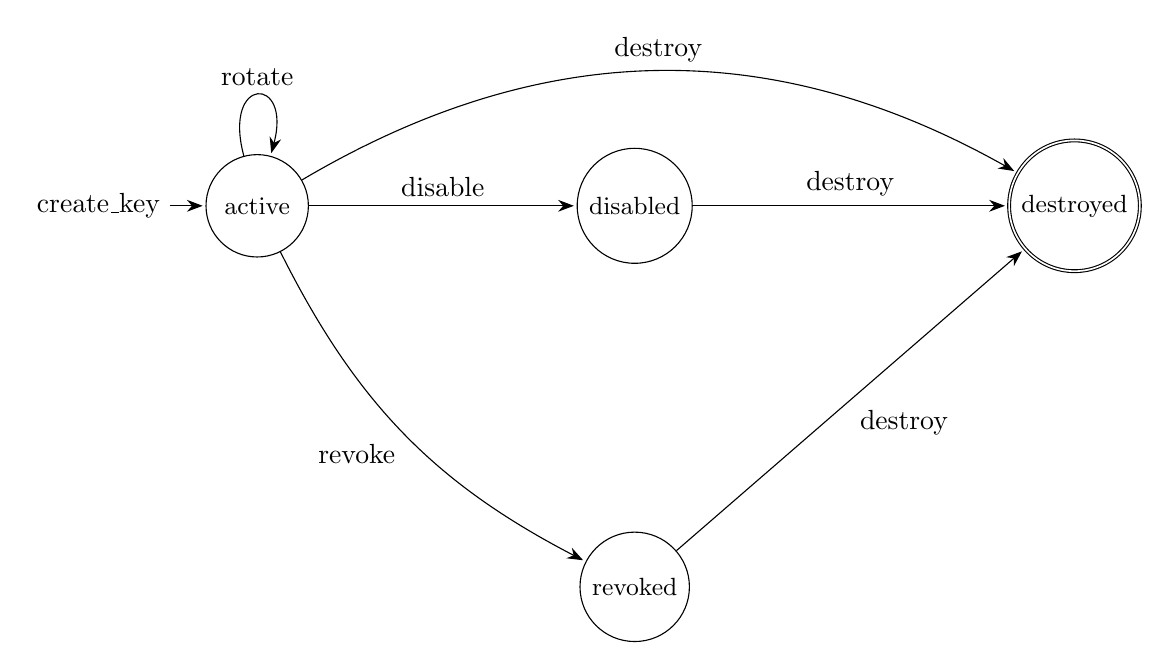
\begin{tikzpicture}[->,>={Stealth[length=2mm]}, shorten >=1pt, auto, node distance=3.4cm,
  every state/.style={draw, font=\small, minimum size=1.3cm}]
  \node[state, initial, initial text={create\_key}] (A)            {active};
  \node[state]            (Di) [right=of A]                        {disabled};
  \node[state]            (R)  [below=of Di]                       {revoked};
  \node[state, accepting] (De) [right=4cm of Di]                   {destroyed};
  \path
    (A)  edge [loop above]      node {rotate}  (A)
    (A)  edge                   node {disable} (Di)
    (A)  edge [bend right=18]   node [swap] {revoke} (R)
    (A)  edge [bend left=30]    node {destroy} (De)
    (Di) edge                   node {destroy} (De)
    (R)  edge                   node [swap] {destroy} (De);
\end{tikzpicture}}
\caption{密钥状态机}
\label{fig:fsm}
\end{figure}

各生命周期操作的设计如下：\textbf{创建}生成随机 DEK 并用主密钥包装，写入 \code{ManagedKey} 与第 1 版 \code{KeyVersion}，响应仅返回元数据；\textbf{轮换}仅允许对 \code{active} 密钥操作，生成新版本 DEK 并递增 \code{key_version}，保留历史版本使旧密文仍可凭版本号解密（SR4）；\textbf{禁用/吊销}将状态置为相应值使密钥不可再用于加解密，二者可对任何非 \code{destroyed} 密钥施加（为简洁，图~\ref{fig:fsm} 主要展示自 \code{active} 出发的路径）；\textbf{销毁}将状态置为 \code{destroyed} 并擦除当前与全部历史版本的包装后密钥材料（SR5），销毁为终态。

\section{安全设计要点汇总}

综合本章设计，系统的安全机制在多个层面落实第~\ref{ch:threat}~章的安全需求：信封加密三层结构加主密钥仅驻留 Enclave（SR1）；每次加密使用新随机 nonce（SR2）；Host$\leftrightarrow$Enclave 远程认证加 AES-GCM 会话加密加序列号防重放（SR8）；JWT 加 RBAC 最小权限（SR7）；关键操作审计（SR6）；解密失败统一错误（SR3）；轮换保留历史版本（SR4）、销毁擦除材料（SR5）。需再次诚实标注两处实现边界：其一，Enclave 用完明文 DEK 后将局部变量重置为零值，但这是受 Python 运行时限制的尽力而为清零；其二，主密钥在 Enclave 中以普通进程内存中的密钥对象形式持有，未经由基类的“加密内存”抽象。这些都是“软件模拟 TEE”定位下的合理取舍。

\section{本章小结}

本章给出了系统的总体设计。围绕“最小可信计算基”与“信封加密分层”两条主线，确立了 Host + Enclave 分离的三层架构（图~\ref{fig:arch}），使密钥策略与密钥材料在物理上分置；设计了主密钥—DEK—业务数据的三层密钥层次（图~\ref{fig:keyhier}、表~\ref{tab:keyhier}），保证数据库仅存包装后的 DEK 与业务密文。在此之上，本章给出了模块划分、双运行模式、数据模型（图~\ref{fig:er}）、API 与权限矩阵（表~\ref{tab:api}）以及密钥生命周期状态机（图~\ref{fig:fsm}），并逐项对应到安全需求 SR1--SR8。其中涉及的关键协议——远程认证握手与加解密全链路时序——将在第~\ref{ch:protocol}~章详细展开。

% ==================== 第 5 章 关键协议与算法实现 ====================
\chapter{关键协议与算法实现}
\label{ch:protocol}

本章详述系统的关键协议与算法实现，包括信封加密、远程认证握手、安全信道、Enclave 内 KMS 操作、密钥轮换以及审计与权限控制。所有描述均对应现有代码，并在涉及安全强度处与第~\ref{ch:threat}~章的边界声明保持一致。

\section{信封加密实现}
\label{sec:envelope-impl}

信封加密是系统密钥保护的核心。其实现分布在 Host 侧（本地模式）与 Enclave 侧（可信模式），二者算法一致，仅执行位置不同。

\textbf{DEK 生成。} 每把受管密钥对应一把随机数据密钥，由 \code{os.urandom(32)}（Enclave 侧为 \code{secure_random(32)}）生成 32 字节随机值。

\textbf{包装（wrap）。} 用主密钥对 DEK 做 AES-256-GCM 加密。实现中生成 12 字节随机 nonce，以固定串 \code{minikms-dek-v1} 作为关联数据（AAD），得到密文与认证标签，最终将密文与 nonce 以 URL-safe Base64 编码后返回。对应核心逻辑为：

\begin{lstlisting}[language=Python]
DEK_ASSOCIATED_DATA = b"minikms-dek-v1"

def wrap_dek(dek: bytes) -> tuple[str, str]:
    nonce = os.urandom(12)
    ciphertext = AESGCM(master_key).encrypt(nonce, dek, DEK_ASSOCIATED_DATA)
    return b64(ciphertext), b64(nonce)
\end{lstlisting}

\textbf{解包（unwrap）。} 用主密钥与相同的 AAD 对包装后的 DEK 做 AES-GCM 解密；若认证标签校验失败（密文被篡改或主密钥不匹配），统一抛出“密钥材料不可用”的通用错误，不泄露内部细节（落实 SR3）。

\textbf{数据加密。} 取得明文 DEK 后，以 DEK 对业务明文做 AES-256-GCM 加密，每次生成新的 12 字节随机 nonce（落实 SR2），并以该密钥的 \code{key_id} 作为 AAD，从而把密文与密钥身份绑定：

\begin{lstlisting}[language=Python]
data_nonce = os.urandom(12)
ciphertext = AESGCM(dek).encrypt(data_nonce, plaintext.encode(), key_id.encode())
\end{lstlisting}

在可信模式下，上述包装、解包与数据加解密\textbf{全部在 Enclave 进程内完成}，明文 DEK 在用完后即被局部置零；Host 只接触包装后的 DEK 与密文。

\section{远程认证协议}
\label{sec:attestation}

可信模式下，Host 启动时与 Enclave 完成一次远程认证握手，建立会话密钥。握手流程如图~\ref{fig:attest} 所示。

\begin{figure}[H]
\centering
\begin{tikzpicture}[font=\footnotesize, >={Stealth[length=2mm]}]
  \node[box] (Hh) at (0,0)  {Host（MiniKMS）};
  \node[box] (Eh) at (8.4,0) {Enclave（KmsEnclave）};
  \draw[dashed] (Hh.south) -- (0,-9.6);
  \draw[dashed] (Eh.south) -- (8.4,-9.6);
  \draw[->] (0,-1.0) -- node[above]{1.~attestation\_request} (8.4,-1.0);
  \draw[<-] (0,-2.1) -- node[above, align=center]{2.~attestation\_response：\\ measurement + identity\_key（明文）} (8.4,-2.1);
  \node[right, text=blue!50!black] at (0.1,-2.9) {3.~校验 measurement = SHA256(code)};
  \draw[->] (0,-3.8) -- node[above]{4.~attestation\_challenge：nonce（32B）} (8.4,-3.8);
  \draw[<-] (0,-4.9) -- node[above, align=center]{5.~attestation\_proof：\\ HMAC(identity\_key, nonce $\Vert$ measurement)} (8.4,-4.9);
  \node[right, text=blue!50!black] at (0.1,-5.7) {6.~校验 HMAC 签名};
  \draw[->] (0,-6.6) -- node[above, align=center]{7.~session\_key\_delivery：\\ Enc$_{\text{identity\_key}}$(session\_key)} (8.4,-6.6);
  \node[left, text=blue!50!black] at (8.3,-7.4) {8.~解密得 session\_key};
  \draw[<-] (0,-8.3) -- node[above]{9.~session\_established（经加密信道）} (8.4,-8.3);
  \draw[<->, very thick] (0,-9.2) -- node[above]{安全信道建立（后续消息 AES-GCM + seq）} (8.4,-9.2);
\end{tikzpicture}
\caption{远程认证握手时序}
\label{fig:attest}
\end{figure}

握手分为身份证明与会话密钥协商两个阶段。前六步中，Enclave 返回其代码度量值（\code{measurement}）与一把身份密钥（\code{identity_key}），Host 先比对度量值是否等于预期常量，再以随机挑战 nonce 要求 Enclave 用身份密钥对 \code{nonce $\Vert$ measurement} 做 HMAC 签名并验证，从而确认对端确实持有该身份密钥且代码度量符合预期；后三步中，Host 生成随机会话密钥，用身份密钥加密后下发，Enclave 解密得到会话密钥，并经由已加密的信道回送确认，握手完成。

需要\textbf{诚实指出其安全边界}：本握手中的 \code{identity_key} 是\textbf{对称密钥且在第 2 步以明文传输}，会话密钥随后用它加密。因此该机制可以拒绝度量值不符或版本错误的 Enclave，但\textbf{不能抵御能够观测并主动操纵握手的攻击者}——这与真实 SGX 中由硬件根证书背书、私钥永不出 Enclave 的非对称远程认证存在本质差异。本文据此将其定位为\textbf{结构性模拟}，其有效性以第~\ref{ch:threat}~章的假设 A-4（本地可信握手信道）为前提。

\section{安全信道}
\label{sec:channel}

握手成功后，Host 与 Enclave 之间的所有消息均通过安全信道传输。信道在传输层采用统一的帧格式：4 字节大端长度前缀加负载。认证阶段的负载为明文 JSON；认证完成后，负载为对 JSON 消息做 AES-256-GCM 加密的结果（密文内含 12 字节 nonce 与 16 字节认证标签）。

为抵御重放攻击，每条加密消息均携带一个单调递增的序列号 \code{seq}：发送方维护 \code{send_seq}，接收方维护期望的 \code{recv_seq}，并在收到消息时校验 \code{seq} 是否等于期望值，不符则判定为重放并拒绝。GCM 的认证标签保证了消息完整性（篡改将导致解密失败），\code{seq} 保证了消息顺序与不可重放，二者共同落实 SR8。

\section{Enclave 内 KMS 操作}
\label{sec:kms-ops}

安全信道建立后，Host 通过三类受保护消息请求 Enclave 完成密钥操作，如表~\ref{tab:kmsmsg} 所示。所有请求与响应均经加密信道传输；明文 DEK 始终不出 Enclave。

\begin{table}[H]
\centering
\caption{Enclave 内 KMS 消息类型}
\label{tab:kmsmsg}
\small
\begin{tabularx}{\textwidth}{L{4.6cm} L{2.0cm} Y}
\toprule
消息类型 & 方向 & 功能 \\
\midrule
\code{kms_generate_wrapped_dek} & Host$\rightarrow$Enclave & 生成随机 DEK 并用主密钥包装，返回包装后的 DEK 与 nonce \\
\code{kms_encrypt} & Host$\rightarrow$Enclave & 解包 DEK 后对明文做 AES-GCM 加密，返回密文与 nonce \\
\code{kms_decrypt} & Host$\rightarrow$Enclave & 解包 DEK 后对密文做 AES-GCM 解密，返回明文 \\
\bottomrule
\end{tabularx}
\end{table}

以加密为例，一次 \code{/crypto/encrypt} 请求的全链路时序如图~\ref{fig:encflow} 所示。Host 在收到客户端请求后，先完成 JWT 鉴权并从数据库读取该密钥当前版本的包装后 DEK，再将密文请求（含 \code{key_id}、包装后 DEK 与待加密明文，\textbf{但不含明文 DEK}）经安全信道转发给 Enclave；Enclave 在内部解包 DEK、完成 AES-GCM 加密、将明文 DEK 局部置零后回送密文；Host 写入审计日志并将结果返回客户端。解密流程与之对称，区别在于 Enclave 执行解密且失败时返回通用错误。

\begin{figure}[H]
\centering
\begin{tikzpicture}[font=\footnotesize, >={Stealth[length=2mm]}]
  \node[box] (Ch) at (0,0)   {Client};
  \node[box] (Hh) at (5.2,0) {Host（MiniKMS）};
  \node[box] (Eh) at (10.6,0){Enclave};
  \draw[dashed] (Ch.south) -- (0,-7.4);
  \draw[dashed] (Hh.south) -- (5.2,-7.4);
  \draw[dashed] (Eh.south) -- (10.6,-7.4);
  \draw[->] (0,-1.0) -- node[above, align=center]{1.~POST /crypto/encrypt\\ \{key\_id, plaintext\} + JWT} (5.2,-1.0);
  \node[right, text=blue!50!black] at (5.3,-1.8) {2.~JWT 鉴权 + 读取包装后 DEK（DB）};
  \draw[->] (5.2,-2.7) -- node[above, align=center]{3.~kms\_encrypt\\ \{key\_id, 包装DEK, plaintext\}} (10.6,-2.7);
  \node[left, text=blue!50!black] at (10.5,-3.5) {4.~解包 DEK $\to$ AES-GCM 加密 $\to$ 置零 DEK};
  \draw[<-] (5.2,-4.4) -- node[above, align=center]{5.~kms\_encrypt\_response\\ \{nonce, ciphertext\}} (10.6,-4.4);
  \node[right, text=blue!50!black] at (5.3,-5.2) {6.~写审计日志（encrypt, success）};
  \draw[<-] (0,-6.1) -- node[above, align=center]{7.~\{key\_id, key\_version,\\ nonce, ciphertext\}} (5.2,-6.1);
\end{tikzpicture}
\caption{加密请求全链路时序（Client $\to$ Host $\to$ Enclave $\to$ Host $\to$ Client）}
\label{fig:encflow}
\end{figure}

\section{密钥轮换}
\label{sec:rotation}

密钥轮换用于限制单把 DEK 的使用时长与数据量。轮换仅允许对 \code{active} 状态的密钥执行：系统生成一把新的 DEK 并用主密钥包装，将密钥的 \code{key_version} 递增，把新版本的包装后 DEK 写入 \code{KeyVersion} 版本表，同时更新主记录的当前版本与轮换时间。关键在于，\textbf{历史版本的包装后 DEK 被保留}，因此使用旧版本加密的历史密文仍可凭其 \code{key_version} 正确解密（落实 SR4）。加密接口始终使用当前版本并在响应中返回 \code{key_version}；解密接口可显式指定 \code{key_version} 以解密历史密文。这一“新数据用新密钥、旧密文仍可解密”的设计在第~\ref{ch:eval}~章的轮换测试中得到验证。

\section{审计与权限控制}
\label{sec:audit-rbac}

\textbf{权限控制。} 系统通过依赖注入实现 RBAC：需要特定角色的接口以 \code{require_roles(...)} 作为依赖，在进入业务逻辑前校验当前用户角色；校验失败返回 403，并记录 \code{permission_denied} 审计事件。普通鉴权接口则以 \code{get_current_user} 校验 JWT 有效性与用户状态。角色与接口的映射关系已在第~\ref{ch:design}~章表~\ref{tab:api} 中给出。

\textbf{审计日志。} 系统对关键操作统一调用审计服务记录事件，字段包括用户、动作、目标类型与 ID、IP、User-Agent、结果与时间。当前记录的动作覆盖登录成功/失败、密钥的创建/查询/轮换/禁用/吊销/销毁、加解密以及越权拒绝等，如表~\ref{tab:auditactions} 所示，为事后追溯与异常检测提供依据（落实 SR6）。

\begin{table}[H]
\centering
\caption{审计记录的关键动作}
\label{tab:auditactions}
\small
\begin{tabularx}{\textwidth}{L{3.0cm} Y}
\toprule
类别 & 动作 \\
\midrule
认证 & \code{login_success}、\code{login_failed} \\
密钥生命周期 & \code{create_key}、\code{rotate_key}、\code{disable_key}、\code{revoke_key}、\code{destroy_key} \\
密钥查询 & \code{list_key_metadata}、\code{get_key_metadata} \\
密码操作 & \code{encrypt}、\code{decrypt} \\
访问控制 & \code{permission_denied}、\code{create_user} \\
\bottomrule
\end{tabularx}
\end{table}

\section{本章小结}

本章详述了系统的关键协议与算法实现。信封加密以 AES-256-GCM 实现 DEK 的包装/解包与数据加解密，并以 AAD 实现用途与身份绑定；远程认证握手在建立会话密钥的同时验证 Enclave 身份，本章如实标注了其作为结构性模拟的安全边界；安全信道以 AES-GCM 加密与序列号防重放保证机密性、完整性与抗重放；Enclave 内 KMS 操作以三类受保护消息完成密钥服务，明文 DEK 始终不出 Enclave（图~\ref{fig:encflow}）；密钥轮换通过版本表兼顾安全性与历史可解密性；审计与 RBAC 共同提供访问控制与可追溯能力。下一章将介绍上述设计的具体实现与部署。

% ==================== 第 6 章 系统实现与部署 ====================
\chapter{系统实现与部署}
\label{ch:impl}

本章介绍系统的具体实现与部署方式，包括技术栈、代码组织、配置与一键启动流程，以及对容器化部署现状的说明。本章所述均对应仓库中的实际文件，便于复现。

\section{技术栈}

系统 Host 侧基于 Python 与 FastAPI 框架实现，主要技术选型如表~\ref{tab:stack} 所示。Enclave 侧除使用 \code{cryptography} 库完成 AES-GCM 加解密外，主要依赖 Python 标准库（\code{socket}、\code{struct}、\code{json}、\code{hashlib}、\code{hmac}）实现通信与认证，依赖较轻，便于审阅与移植。

\begin{table}[H]
\centering
\caption{主要技术栈}
\label{tab:stack}
\small
\begin{tabularx}{\textwidth}{L{3.6cm} Y}
\toprule
方面 & 选型 \\
\midrule
语言与运行时 & Python 3.12 \\
Web 框架 & FastAPI（自带 Swagger / OpenAPI 文档） \\
ORM 与数据库 & SQLAlchemy 2.x；默认 SQLite，可通过 \code{DATABASE_URL} 迁移至 PostgreSQL \\
身份认证 & JWT Bearer 令牌（PyJWT），HMAC-SHA256 签名 \\
口令哈希 & bcrypt \\
密码学 & \code{cryptography} 库，AES-256-GCM \\
Host$\leftrightarrow$Enclave 通信 & TCP（环回）或 Unix Domain Socket \\
测试 & pytest 与 FastAPI TestClient \\
\bottomrule
\end{tabularx}
\end{table}

\section{代码组织}

项目位于多项目工作区下，Host 侧与 Enclave 侧分置于两个目录，核心结构如下：

\begin{lstlisting}[language={}]
20_安全应用与实验/
|-- start-trusted-kms.sh          # 一键启动（Enclave + API）
|-- 密钥管理系统/                  # Host 侧（FastAPI / MiniKMS）
|   |-- app/
|   |   |-- main.py               # 应用入口，lifespan 连接 Enclave
|   |   |-- config.py             # USE_ENCLAVE / MASTER_KEY / ENCLAVE_PORT
|   |   |-- api/                  # auth, users, keys, crypto, audit 路由
|   |   |-- services/             # 鉴权、密钥、加解密、审计、Enclave 客户端
|   |   |-- models/               # ORM：user, key, audit_log
|   |   |-- schemas/              # Pydantic 请求/响应模型
|   |   `-- utils/                # security(JWT/bcrypt), permissions(RBAC)
|   |-- tests/                    # test_minikms_api.py / test_trusted_kms.py
|   `-- docs/                     # 设计文档、论文大纲与初稿
`-- 机密计算/                      # Enclave 侧
    `-- src/
        |-- kms_enclave.py        # KMS 专用 Enclave（持有主密钥）
        |-- enclave.py            # TEE 基类（认证、信道、密封存储）
        `-- crypto.py             # AES-GCM、HMAC、measure_code
\end{lstlisting}

这一组织与第~\ref{ch:design}~章的模块划分（表~\ref{tab:modules}）一一对应：API 路由层薄、服务层承载业务逻辑、密码学后端通过 \code{enclave_client} 与 Enclave 解耦，使本地模式与可信模式得以共享同一套上层代码。

\section{配置与部署}

\subsection{配置项}

系统通过环境变量（或 \code{.env} 文件）配置，关键项包括：\code{JWT_SECRET_KEY}（JWT 签名密钥）、\code{DATABASE_URL}（数据库连接串）、\code{USE_ENCLAVE}（运行模式开关）、\code{ENCLAVE_PORT} 或 \code{ENCLAVE_SOCKET_PATH}（Enclave 通信地址），以及仅在本地模式下需要的 \code{MASTER_KEY}。其中主密钥须为 Base64 编码的 32 字节值，可由如下命令生成：

\begin{lstlisting}[language=bash]
python -c "import base64, os; print(base64.urlsafe_b64encode(os.urandom(32)).decode())"
\end{lstlisting}

如第~\ref{ch:design}~章所述，当 \code{USE_ENCLAVE=true} 时，配置层会强制忽略 Host 上的 \code{MASTER_KEY}，确保主密钥仅注入 Enclave 进程（落实 SR1）。

\subsection{一键启动}

为便于演示与复现，系统提供一键启动脚本 \code{start-trusted-kms.sh}。脚本自动从 \code{密钥管理系统/.env} 读取 \code{MASTER_KEY} 并\textbf{仅传递给 Enclave 进程}，随后以可信模式启动 Enclave 与 API，并打开 Swagger 文档：

\begin{lstlisting}[language=bash]
cd "/Users/.../20_安全应用与实验"
./start-trusted-kms.sh
# API 默认 http://127.0.0.1:8000/docs
# 可选：API_PORT=8001 ENCLAVE_PORT=9788 ./start-trusted-kms.sh
\end{lstlisting}

启动后可通过健康检查接口 \code{GET /} 确认系统处于可信模式且 Enclave 已连接：

\begin{lstlisting}[language={}]
{
  "service": "TrustedKMS",
  "status": "ok",
  "crypto_backend": "enclave",
  "enclave": "connected"
}
\end{lstlisting}

其中 \code{crypto_backend} 为 \code{enclave} 表示加解密由 Enclave 后端承载，\code{enclave} 为 \code{connected} 表示远程认证握手已成功、安全信道已建立。应用入口在 \code{lifespan} 中于启动时调用 \code{connect_and_attest()} 完成握手，并在关闭时释放连接。

\subsection{手动启动}

在需要分别观察两个进程时，也可手动启动：在一个终端中为 Enclave 设置 \code{MASTER_KEY} 与 \code{ENCLAVE_PORT} 并运行 \code{python -m src.kms_enclave}；在另一个终端中为 Host 设置 \code{USE_ENCLAVE=true} 与相同的 \code{ENCLAVE_PORT}（且\textbf{不设置} \code{MASTER_KEY}）并以 uvicorn 启动 API。此方式直观地体现了主密钥仅存在于 Enclave 进程这一设计。

\section{容器化部署现状}

仓库中提供了用于 Host 的 \code{Dockerfile} 与 \code{docker compose} 配置，可将 API 容器化运行。但需\textbf{诚实说明}：当前容器化仅覆盖 Host 侧，尚未将 Enclave 拆分为独立容器，因此可信模式的标准部署方式仍以本节的一键脚本（本机双进程）为主。将 Enclave 独立容器化、并在容器边界上重新审视信任假设，列入第~\ref{ch:conclusion}~章的未来工作。

\section{本章小结}

本章介绍了系统的实现与部署。系统以 Python/FastAPI 实现 Host 侧、以轻量依赖实现 Enclave 侧，代码组织与设计章节的模块划分一致；通过环境变量切换运行模式，并以一键启动脚本完成 Enclave 与 API 的联合部署与健康检查。本章亦如实说明了容器化部署目前仅覆盖 Host 侧这一现状。下一章将基于该实现开展测试与实验评估。

% ==================== 第 7 章 测试与实验评估 ====================
\chapter{测试与实验评估}
\label{ch:eval}

本章通过自动化测试与分析性评估验证系统是否满足第~\ref{ch:threat}~章的安全需求与功能目标。内容包括测试策略、功能测试、安全属性验证、性能评估设计以及与云 KMS 的定性对比。为遵循“不虚构未实现功能”的原则，本章明确区分\textbf{已由测试验证}的结论与\textbf{设计级/待测}的结论。

\section{测试策略}

系统采用基于 pytest 与 FastAPI TestClient 的自动化测试，分为两组：本地模式的 API 测试（\code{tests/test_minikms_api.py}）与可信模式的集成测试（\code{tests/test_trusted_kms.py}）。后者在测试内启动一个真实的 \code{KmsEnclave} 线程并通过环回 TCP 连接，因此可端到端地验证远程认证、安全信道与 Enclave 后端加解密。两组共 8 个测试用例，最近一次运行结果为全部通过（8 passed）。

\section{功能测试}

8 个测试用例及其验证内容与关联需求如表~\ref{tab:tests} 所示。

\begin{table}[H]
\centering
\caption{功能测试用例}
\label{tab:tests}
\footnotesize
\begin{tabularx}{\textwidth}{c Y L{3.0cm}}
\toprule
\# & 测试用例与验证内容 & 关联需求 \\
\midrule
1 & 首个注册用户自动成为 Admin，可登录并访问 \code{/auth/me} & 鉴权 \\
2 & 口令以 bcrypt 哈希存储（以 \code{\$2} 开头），非明文 & T7 \\
3 & Admin 可创建用户；App User 创建密钥被拒（403），审计含 \code{permission_denied} & SR7 / T6 \\
4 & 创建与加解密往返；响应不含密钥材料；禁用/吊销后拒绝加解密；销毁后数据库中包装材料被擦空 & SR3 / SR5 / T1 \\
5 & 轮换后版本号递增为 2；新旧版本密文均可正确解密 & SR4 \\
6 & 审计记录登录成功/失败、创建/查询密钥、加密、销毁等动作 & SR6 \\
7 & 可信模式加解密往返一致；健康检查 \code{crypto_backend=enclave}、\code{enclave=connected} & SR1 / SR8 \\
8 & 可信模式轮换后仍可解密旧版本密文 & SR4 \\
\bottomrule
\end{tabularx}
\end{table}

用例 7 与 8 尤为关键：它们在真实启动的 Enclave 与已建立的安全信道之上完成加解密往返与跨版本解密，从而端到端地验证了远程认证、AES-GCM 信道与 Enclave 后端的联通与正确性，对应可信模式的核心设计。

\section{安全属性验证}

在功能测试之外，本节对关键安全属性作进一步说明，并标注其验证层级。

\begin{itemize}
  \item \textbf{主密钥不在 Host（SR1）。} 可信模式下配置层强制将 Host 的 \code{master_key} 置空（见第~\ref{ch:design}~章），可信集成测试的运行环境亦显式删除了 Host 的 \code{MASTER_KEY} 环境变量；健康检查显示 \code{crypto_backend=enclave}，加解密由 Enclave 承载。\emph{（测试 + 设计验证）}
  \item \textbf{数据库不含明文密钥材料（T1/SR5）。} 测试断言密钥创建与查询响应中不含 \code{encrypted_key_material} 与 \code{nonce} 字段；销毁后直接查询数据库确认包装材料已被置空。\emph{（测试验证）}
  \item \textbf{密文完整性（T4）。} AES-GCM 的认证标签在设计上保证任何对密文的篡改都会导致解密失败；当前测试覆盖了状态非法（禁用/吊销）导致的解密拒绝，\textbf{尚未包含针对密文比特翻转的专门篡改用例}，可作为测试补强项。\emph{（设计验证）}
  \item \textbf{统一错误（SR3）。} 解包与解密失败均返回通用错误信息，不泄露内部异常细节。\emph{（设计 + 用例 4 间接验证）}
\end{itemize}

\section{性能评估设计}

为量化将敏感操作迁移至 Enclave 所引入的进程间通信（IPC）开销，可设计本地模式与可信模式的延迟对比实验：在相同负载下分别测量创建密钥、加密、解密三类操作的延迟，并统计 P50 与 P95。实验设计如表~\ref{tab:perf} 所示。

\begin{table}[H]
\centering
\caption{性能对比实验设计（本地模式 vs.\ 可信模式）}
\label{tab:perf}
\small
\begin{tabularx}{\textwidth}{L{3.2cm} C{2.4cm} C{2.4cm} Y}
\toprule
操作 & 本地 P50/P95 & 可信 P50/P95 & 说明 \\
\midrule
创建密钥 & ---\,/\,--- & ---\,/\,--- & 含一次 \code{kms_generate_wrapped_dek} \\
加密 & ---\,/\,--- & ---\,/\,--- & 含一次 \code{kms_encrypt} \\
解密 & ---\,/\,--- & ---\,/\,--- & 含一次 \code{kms_decrypt} \\
\bottomrule
\end{tabularx}
\end{table}

需\textbf{诚实说明}：本文当前未提供该实验的实测数值，表~\ref{tab:perf} 仅给出实验设计与待填栏位。从原理上预期可信模式因增加了一次本地 IPC 往返与一次会话层 AES-GCM 加解密，单次操作延迟将略高于本地模式，但二者均应处于可接受范围；具体数值留待后续补充。

\section{与云 KMS 的对比讨论}

本文系统在定位上是教学/研究原型，与生产级云 KMS 存在显著差异，定性对比如表~\ref{tab:cloudkms} 所示。对比的目的不在于宣称本文系统达到生产水平，而在于厘清其适用边界。

\begin{table}[H]
\centering
\caption{本文系统与云 KMS 的定性对比}
\label{tab:cloudkms}
\small
\begin{tabularx}{\textwidth}{L{3.0cm} Y Y}
\toprule
维度 & 本文系统 & 生产级云 KMS \\
\midrule
密钥隔离 & 软件模拟 Enclave（进程级） & HSM / 硬件 TEE（硬件级） \\
远程认证 & 结构性模拟（对称、明文身份密钥） & 硬件根信任、非对称、厂商背书 \\
高可用 & 单实例，无集群 & 多副本、跨区域高可用 \\
功能完整度 & 信封加密、生命周期、RBAC、审计 & 上述功能 + 合规、审批流、配额等 \\
适用场景 & 教学、研究、原型演示 & 生产环境密钥托管 \\
\bottomrule
\end{tabularx}
\end{table}

\section{本章小结}

本章通过 8 个自动化测试用例验证了系统在本地模式与可信模式下的鉴权、密钥生命周期、加解密往返、密钥轮换与审计等功能的正确性，其中可信模式用例端到端地验证了远程认证、安全信道与 Enclave 后端的联通。本章进一步分析了关键安全属性，并诚实标注了测试覆盖的边界（如密文篡改专项用例待补强）。在性能方面，本章给出了本地与可信模式的对比实验设计，但未提供实测数值。最后，本章通过与云 KMS 的定性对比厘清了系统的适用边界。

% ==================== 第 8 章 总结与展望 ====================
\chapter{总结与展望}
\label{ch:conclusion}

\section{工作总结}

本文围绕“在 Host 不可信前提下保护密钥敏感操作”这一核心问题，设计并实现了一套 Host 与 Enclave 分离的轻量级密钥管理系统，主要工作包括：

\begin{enumerate}
  \item \textbf{架构与密钥层次。} 提出并实现了 Host + Enclave 分离的三层架构，以信封加密构建“主密钥—数据密钥—业务数据”的层次结构，使主密钥仅驻留于模拟 Enclave，数据库仅保存包装后的 DEK 与业务密文。
  \item \textbf{协议实现。} 实现了 Host 与 Enclave 之间的远程认证握手与基于 AES-256-GCM、带序列号防重放的安全信道，并在 Enclave 内完成 DEK 的包装/解包与数据加解密，使明文 DEK 不出 Enclave。
  \item \textbf{系统功能。} 实现了 JWT 鉴权、基于角色的访问控制、版本化密钥轮换、密钥全生命周期管理与审计日志，并提供本地与可信两种可对照的运行模式。
  \item \textbf{威胁模型与验证。} 建立了系统的威胁模型与安全需求（SR1--SR8），逐项给出已实现的缓解机制，并诚实界定了软件模拟 TEE 的能力边界；以 8 项自动化集成测试验证了系统在两种模式下的功能正确性，并提供一键启动以保证可复现。
\end{enumerate}

综上，在“Host 不可信、Enclave 相对可信”的受控威胁模型下，本文方案能够将主密钥与数据密钥的敏感操作隔离至 Enclave，达成了既定研究目标。

\section{局限性}

本着诚实表述的原则，本文系统存在以下局限，这些局限与第~\ref{ch:threat}~章的边界声明一致：

\begin{itemize}
  \item \textbf{软件模拟而非硬件隔离。} Enclave 为普通操作系统进程，主密钥驻留于普通进程内存，不具备硬件内存加密与隔离，无法抵御物理攻击、内存转储与 Enclave 自身被攻破等威胁。
  \item \textbf{远程认证为结构性模拟。} 身份密钥为对称密钥且握手阶段以明文传输，缺乏硬件根信任，无法抵御对握手过程的主动中间人攻击，其有效性依赖本地可信握手信道这一假设。
  \item \textbf{授权粒度与多租户。} 访问控制为角色级，任意已鉴权用户可使用任意 active 密钥，缺乏逐密钥 ACL 与租户隔离。
  \item \textbf{工程完整度。} 仍使用 SQLite、单 Enclave 实例、无高可用集群；容器化仅覆盖 Host 侧；未实现传输层 TLS（依赖部署层）、令牌吊销与自动轮换策略。
  \item \textbf{未做形式化验证。} 远程认证与信道协议未经过形式化建模与证明，性能也尚未给出实测数据。
\end{itemize}

\section{未来工作}

针对上述局限，后续可在以下方向展开：

\begin{enumerate}
  \item \textbf{对接真实硬件 TEE。} 将模拟 Enclave 替换为 Intel SGX 或 AWS Nitro Enclaves，采用硬件根信任的非对称远程认证，从根本上提升隔离强度。
  \item \textbf{后量子密钥封装。} 引入 ML-KEM 等后量子算法\cite{fips203}，对 DEK 的封装采用经典与后量子混合方案，提升前瞻安全性。
  \item \textbf{工程化增强。} 迁移至 PostgreSQL 并引入数据库迁移；实现密钥审批流、自动轮换策略、令牌吊销与多租户隔离；将 Enclave 独立容器化部署。
  \item \textbf{形式化与性能。} 对远程认证与安全信道协议进行形式化建模与分析；补充本地与可信模式的性能对比实测，量化 Enclave IPC 开销。
  \item \textbf{管理与演示界面。} 提供管理后台与可视化演示，提升系统可用性与展示效果。
\end{enumerate}

总体而言，本文完成了一个定位清晰、边界诚实、可复现的应用密码学工程原型，为后续对接真实 TEE 与后量子密钥封装提供了可扩展的基础。


% ---------------- 参考文献 ----------------
% ==================== 参考文献 ====================
\begin{thebibliography}{99}
\addcontentsline{toc}{chapter}{参考文献}

\bibitem{nist80057} Barker E. Recommendation for Key Management, Part 1: General. NIST Special Publication 800-57 Part 1 Revision 5, 2020.

\bibitem{fips197} National Institute of Standards and Technology. Advanced Encryption Standard (AES). FIPS PUB 197, 2001.

\bibitem{dworkin2007gcm} Dworkin M. Recommendation for Block Cipher Modes of Operation: Galois/Counter Mode (GCM) and GMAC. NIST Special Publication 800-38D, 2007.

\bibitem{mcgrew2004gcm} McGrew D, Viega J. The Security and Performance of the Galois/Counter Mode (GCM) of Operation. In: Proceedings of INDOCRYPT, 2004: 343--355.

\bibitem{rogaway2002aead} Rogaway P. Authenticated-Encryption with Associated-Data. In: Proceedings of the 9th ACM Conference on Computer and Communications Security (CCS), 2002: 98--107.

\bibitem{rfc5116} McGrew D. An Interface and Algorithms for Authenticated Encryption. RFC 5116, IETF, 2008.

\bibitem{rfc2104} Krawczyk H, Bellare M, Canetti R. HMAC: Keyed-Hashing for Message Authentication. RFC 2104, IETF, 1997.

\bibitem{fips180} National Institute of Standards and Technology. Secure Hash Standard (SHS). FIPS PUB 180-4, 2015.

\bibitem{rfc7519} Jones M, Bradley J, Sakimura N. JSON Web Token (JWT). RFC 7519, IETF, 2015.

\bibitem{provos1999bcrypt} Provos N, Mazi\`eres D. A Future-Adaptable Password Scheme. In: Proceedings of the USENIX Annual Technical Conference, 1999.

\bibitem{rfc8018} Moriarty K, Kaliski B, Rusch A. PKCS \#5: Password-Based Cryptography Specification Version 2.1. RFC 8018, IETF, 2017.

\bibitem{sabt2015tee} Sabt M, Achemlal M, Bouabdallah A. Trusted Execution Environment: What It is, and What It is Not. In: IEEE Trustcom/BigDataSE/ISPA, 2015: 57--64.

\bibitem{costan2016sgx} Costan V, Devadas S. Intel SGX Explained. IACR Cryptology ePrint Archive, Report 2016/086, 2016.

\bibitem{mckeen2013sgx} McKeen F, Alexandrovich I, Berenzon A, et al. Innovative Instructions and Software Model for Isolated Execution. In: Proceedings of the 2nd International Workshop on Hardware and Architectural Support for Security and Privacy (HASP), 2013.

\bibitem{anati2013attestation} Anati I, Gueron S, Johnson S, Scarlata V. Innovative Technology for CPU Based Attestation and Sealing. In: Proceedings of HASP, 2013.

\bibitem{pinto2019trustzone} Pinto S, Santos N. Demystifying Arm TrustZone: A Comprehensive Survey. ACM Computing Surveys, 2019, 51(6): 1--36.

\bibitem{fips203} National Institute of Standards and Technology. Module-Lattice-Based Key-Encapsulation Mechanism Standard. FIPS PUB 203, 2024.

\end{thebibliography}


% ---------------- 附录 ----------------
\appendix
% ==================== 附录 ====================
% 进入附录前 main.tex 已调用 \appendix；此处仅配置编号样式。
\ctexset{ chapter/name = {附录\ ,}, chapter/number = \Alph{chapter} }

\chapter{主要 API 请求/响应示例}
\label{app:api}

以下示例省略了 JWT 令牌等头部，仅示意请求体与响应体（实际响应字段以代码为准）。

\textbf{A.1 注册与登录}
\begin{lstlisting}[language={}]
POST /auth/register
{ "username": "admin", "email": "admin@example.com", "password": "Password123!" }
--> 201 { "id": 1, "username": "admin", "role": "admin", "status": "active" }

POST /auth/login
{ "username": "admin", "password": "Password123!" }
--> 200 { "access_token": "<JWT>", "token_type": "bearer" }
\end{lstlisting}

\textbf{A.2 创建密钥（响应不含任何密钥材料）}
\begin{lstlisting}[language={}]
POST /keys
{ "key_name": "demo-key", "expires_at": null }
--> 201 {
  "id": "f3c1...uuid", "key_name": "demo-key", "key_type": "AES-256-GCM",
  "key_status": "active", "key_version": 1
}
\end{lstlisting}

\textbf{A.3 加密与解密往返}
\begin{lstlisting}[language={}]
POST /crypto/encrypt
{ "key_id": "f3c1...uuid", "plaintext": "hello Trusted KMS" }
--> 200 { "key_id": "f3c1...uuid", "key_version": 1,
          "nonce": "<b64>", "ciphertext": "<b64>" }

POST /crypto/decrypt
{ "key_id": "f3c1...uuid", "nonce": "<b64>", "ciphertext": "<b64>" }
--> 200 { "plaintext": "hello Trusted KMS" }
\end{lstlisting}

\chapter{远程认证与 KMS 消息 JSON 格式}
\label{app:proto}

\textbf{B.1 远程认证握手消息}
\begin{lstlisting}[language={}]
Host  -> { "type": "attestation_request" }
Enc   -> { "type": "attestation_response",
           "measurement": "<hex>", "identity_key": "<hex>" }   # 明文
Host  -> { "type": "attestation_challenge", "nonce": "<hex 32B>" }
Enc   -> { "type": "attestation_proof", "signature": "<hex>" }  # HMAC
Host  -> { "type": "session_key_delivery", "encrypted_key": "<hex>" }
Enc   -> { "type": "session_established" }                      # 经加密信道
\end{lstlisting}

\textbf{B.2 KMS 操作消息（均经 AES-GCM 安全信道，含 seq）}
\begin{lstlisting}[language={}]
Host  -> { "type": "kms_generate_wrapped_dek" }
Enc   -> { "type": "kms_generate_wrapped_dek_response",
           "encrypted_key_material": "<b64>", "nonce": "<b64>" }

Host  -> { "type": "kms_encrypt", "key_id": "...",
           "encrypted_key_material": "<b64>", "key_nonce": "<b64>",
           "plaintext": "..." }
Enc   -> { "type": "kms_encrypt_response", "nonce": "<b64>", "ciphertext": "<b64>" }

Host  -> { "type": "kms_decrypt", "key_id": "...",
           "encrypted_key_material": "<b64>", "key_nonce": "<b64>",
           "nonce": "<b64>", "ciphertext": "<b64>" }
Enc   -> { "type": "kms_decrypt_response", "plaintext": "..." }
\end{lstlisting}

\chapter{核心代码片段}
\label{app:code}

以下片段摘自实际代码并略作精简（去除部分日志与注释），用于说明核心逻辑。

\textbf{C.1 信封加密：DEK 的包装与解包（Enclave 侧）}
\begin{lstlisting}[language=Python]
DEK_ASSOCIATED_DATA = b"minikms-dek-v1"

def _wrap_dek(self, dek):
    nonce = secure_random(12)
    ciphertext = self._master_aesgcm.encrypt(nonce, dek, DEK_ASSOCIATED_DATA)
    return b64(ciphertext), b64(nonce)

def _unwrap_dek(self, encrypted_key_material, nonce):
    enc = b64decode(encrypted_key_material)
    nonce_bytes = b64decode(nonce)
    return self._master_aesgcm.decrypt(nonce_bytes, enc, DEK_ASSOCIATED_DATA)
\end{lstlisting}

\textbf{C.2 Enclave 内加密（明文 DEK 用完即置零）}
\begin{lstlisting}[language=Python]
def _handle_encrypt(self, conn, msg):
    dek = self._unwrap_dek(msg["encrypted_key_material"], msg["key_nonce"])
    data_nonce = secure_random(12)
    ciphertext = AESGCM(dek).encrypt(
        data_nonce, msg["plaintext"].encode(), msg["key_id"].encode())
    dek = b"\x00" * 32  # best-effort zeroization (受 Python 运行时限制)
    self._send_secure(conn, {
        "type": "kms_encrypt_response",
        "nonce": b64(data_nonce), "ciphertext": b64(ciphertext)})
\end{lstlisting}

\textbf{C.3 远程认证握手（Host 侧，精简）}
\begin{lstlisting}[language=Python]
send_raw({"type": "attestation_request"})
msg = recv_raw()
measurement  = bytes.fromhex(msg["measurement"])
identity_key = bytes.fromhex(msg["identity_key"])
assert measurement == expected_measurement      # 校验度量值

challenge = secure_random(32)
send_raw({"type": "attestation_challenge", "nonce": challenge.hex()})
proof = recv_raw()
assert hmac_verify(identity_key, challenge + measurement,
                   bytes.fromhex(proof["signature"]))   # 校验 HMAC

session_key = secure_random(32)
enc = aes_gcm_encrypt(identity_key, session_key)
send_raw({"type": "session_key_delivery", "encrypted_key": enc.hex()})
assert recv_secure()["type"] == "session_established"
\end{lstlisting}

\chapter{测试与运行截图}
\label{app:screens}

本附录预留运行截图位置，建议插入：Swagger 接口文档、健康检查响应、审计日志查询，以及 \code{pytest} 全部用例通过（8 passed）的输出。

\begin{figure}[H]
\centering
\fbox{\begin{minipage}[c][4.5cm][c]{0.8\textwidth}\centering\itshape
（此处插入截图：Swagger / 健康检查 / 审计日志 / pytest 8 passed）
\end{minipage}}
\caption{运行截图（占位，待插入）}
\label{fig:screens}
\end{figure}


\end{document}
